\documentclass[a4paper]{article}
\usepackage[dutch]{babel}
\usepackage[utf8]{inputenc}
\usepackage{titling}
\usepackage{url}
\usepackage{booktabs}
\usepackage{pgfplots}
\usepackage{float}
\usepackage[section]{placeins}
\usepackage{subcaption}
\usepackage{textcomp}
\usepackage{amsmath}
\usepackage{mathtools}

\pgfplotsset{minor tick style={thin}}
\numberwithin{equation}{section}

\begin{document}
    \graphicspath{ {./images/} }

    \begin{titlepage}
    \newpage
    \thispagestyle{empty}
    \frenchspacing
    \hspace{-0.2cm}
    
\includegraphics[height=3.4cm]{sedes}
    \hspace{0.2cm}
    \rule{0.5pt}{3.4cm}
    \hspace{0.2cm}
    \begin{minipage}[b]{8cm}
        \Large{Katholieke\newline Universiteit\newline Leuven}\smallskip\newline
        \large{}\smallskip\newline
        \textbf{Department of\newline Computer Science}\smallskip
    \end{minipage}
    \hspace{\stretch{1}}
    \vspace*{3.2cm}\vfill
    \begin{center}
        \begin{minipage}[t]{\textwidth}
            \begin{center}
                \LARGE{\rm{\textbf{\uppercase{Gegevensstructuren en Algoritmen:}}}}\\
                \Large{\rm{Practicum 2}}
            \end{center}
        \end{minipage}
    \end{center}
    \vfill
    \hfill\makebox[8.5cm][l]{%
        \vbox to 7cm{\vfill\noindent
            {\rm\textbf{Mats Fockaert r0695565}}\\
            {\rm Academic year 2020--2021}
            
        }
    }
\end{titlepage}


    \tableofcontents
    \listoffigures
    \listoftables

    \pagebreak
    \section{Inleiding}
        Het probleem dat we willen bekijken is het 8-puzzel probleem. 
        We willen een algoritme maken dat efficiënt en eindig is. 
        Wanneer een puzzel niet oplosbaar is, willen we dit meteen weten en dit melden.
        \\
        \\We doen dit a.d.h.v. A*. Dit is een kortste pad algoritme die m.b.v. enkele heuristieken probeert zo snel mogelijk een oplossing te vinden.

    \section{Methode}
        Zoals eerder vermeld gebruiken we enkele heuristieken, namenlijk, de hammingfunctie en de manhattanfunctie.
        De hammingfunctie telt het aantal tegels die fout staan en de manhattanfunctie telt het aantal vakjes nodig om een tegel op de correcte plaats te zetten.
        Bij beide functies tellen het aantal verschuivingen om bij de toestand te geraken ook mee.
        Deze bereken een kost bij een bordpositie waaruit we een prioriteit kunnen opstellen.
        Hiervoor maken we gebruik van een prioriteitsrij die alle borden a.d.h.v. hun heuristieke kost sorteert.
        De prioriteitsrij wordt geinitialiseerd met het start bord. Dan worden alle buurposities -- posities die te bereiken zijn door \'e\'en tegel te verschuiven -- in de rij opgeslagen.
        Het bord aan het begin van de rij heeft nu de laagste kost, deze nemen we uit de rij en herhalen het proces.
        \\
        \\Enkele optimalisaties aan A* voor dit probleem:
        \begin{itemize}
            \item we berekenen bij de start van het algoritme of het beginbord wel effectief oplosbaar is,
            \item we kijken bij het zoeken naar buren of deze al voorkwamen bij het huidige bord zijn voorganger, zo niet, voegen we de buur toe aan de rij.
        \end{itemize}

    \pagebreak

    \section{Resultaten}
        \begin{table}[!ht]
            \centering
            \begin{tabular}{r r r r}
                \toprule
                \multicolumn{1}{l}{Puzzel} & \multicolumn{1}{l}{Aantal verplaatsingen} & \multicolumn{1}{l}{Uitvoeringstijd} &\\
                & &\multicolumn{1}{l}{Hamming}& \multicolumn{1}{l}{Manhattan} \\
                \midrule
                puzzle28.txt & $28$ & $1.533$ & $0.044$\\
                puzzle30.txt & $30$ & $3.375$ & $0.055$\\
                puzzle32.txt & $32$ & $/$ & $2.170$\\
                puzzle34.txt & $34$ & $/$ & $0.472$\\
                puzzle36.txt & $36$ & $/$ & $4.272$\\
                puzzle38.txt & $38$ & $/$ & $50.830$\\
                puzzle40.txt & $40$ & $/$ & $48.224$\\
                puzzle42.txt & $42$ & $/$ & $74.591$\\
                \bottomrule
            \end{tabular}
            \caption[Prestatie van het A* algoritme.]{Bevat het minimum aantal verplaatsingen om de doeltoestand te bereiken en,
               de uitvoeringstijd (in seconden) van het A* algoritme voor de Hamming en de Manhattan
                prio-riteitsfuncties. Wanneer een oplossing niet binnen een redelijke
                tijd ($< 5$ minuten) gevonden kan worden, staat er een $/$.}
            \label{tab:Prestatie A*}
        \end{table}

    \pagebreak

    \section{Bespreking van de resultaten}
        \subsection{Complexiteit van de prioriteitsfuncties}
            \textbf{De hammingfunctie} moet voor elk vak beslissen of het correct geplaatst is in de puzzel.
            \\\textbf{De manhattanfunctie} moet voor elk vak kijken hoeveel vakken een tegel fout staat.
            Bij beide gaan we dus naar elk vak moeten kijken of het al dan niet fout is. 
            \\Voor een bord van grootte $N$ hebben we 
            $N \times N$ arrayelementen. We moeten dus $N^2$ keer over het bord gaan. De complexiteit is dus voor beide $\sim N^2$.
           
        \pagebreak

        \subsection{Implementatie isSolvable}
        De oplosbaarheid berekenen gebeurt als volgt:
        \begin{enumerate}
            \item Vind het lege vak. Hiervoor moeten we heel het bord afgaan. Stel we hebben een bord van grootte $N$ dan moeten we $N^2$ elementen afgaan.
            Gemiddeld is dit $\frac{N^2}{2}$ elementen.
            \item Zorg ervoor dat het gegeven bord zijn nulvak in de rechteronderhoek bevindt. Om het gemiddelde te berekenen, kijken we naar het beste en slechtste geval:
            \begin{itemize}
                \item In het beste geval, staat het lege vak reeds correct en zijn er $0$ verschuivingen nodig.
                \item In het slechtste geval, staat het lege vak in de linkse bovenhoek. We hebben dan, voor een bord van grootte $N$, $N - 1$ verplaatsingen naar beneden en naar rechts nodig. Dit geeft $2(N-1)$ verplaatsingen.
            \end{itemize}
            Gemiddeld geeft dit dan $N - 1$ verplaatsingen. De functie gaat \'e\'en rijtoegang voor het nulvak, \'e\'en voor het te verwisselen vak en \'e\'en voor de wissel zelf nodig hebben. Dit geeft $3$ rijtoegangen per wissel. We hebben dus $3N-3$ rijtoegangen.
            \item Het opslaan van de nieuwe plaatsen. Het hele bord wordt hiervoor afgelopen, en de locatie wordt voor elk element (behalve het lege) in een nieuwe rij gestoken.  Dit geeft een totaal van $2N^2 \-- 1$ aantal rijtoegangen.
            \item Voer de volgende functie uit gebruikmakende van een hulpfunctie die de positie van elk gevraagd cijfer teruggeeft:
            \begin{equation}
                oplosbaar(b) = \frac{\prod_{i<j} (p(b, j)-p(b, i))}{\prod_{i<j}(j-i)},
            \end{equation}
            De formule zal $\frac{N(N-1)}{2}$ keer opgeroepen kunnen worden. Hiervoor moeten we per keer twee elementen opvragen wat dus voor $N(N-1)$ rijtoegangen zorgt.  
            \item Kijk of oplosbaar(b) een resultaat dat $\geq 0$ teruggeeft, dan is het oplosbaar.
        \end{enumerate}
        Wanneer we dit alles optellen, krijgen we de uiteindelijke tijdscomplexiteit van de solver:
        \begin{align*}
            \frac{N^2}{2} + 3N -3 + 2N^2 - 1 + N(N-1) = 3N^2 + \frac{N^2}{2} +2N -4 \rightarrow \sim 3N^2
        \end{align*}
        
            
    \pagebreak

        \subsection{Geheugengebruik}
        Om de borden te onderzoeken, slaan we deze iteratief op in een rij. Wegens de isSolvable methode weten we dat niet alle bordposities opgeslagen zullen worden. 
        Namenlijk, het resultaat van isSolvable van een bepaald bord kan of positief zijn, of negatief zijn. Van alle mogelijke borden, moeten we dus maar de helft effectief opslaan.
        Neem een bord van grootte $N$, dit bord heeft $N \times N$ elementen en dus $N^2!$ aantal mogelijke bordposities. Net hebben we aangetoond dat we maar naar $\frac{1}{2}$ posities moeten kijken omdat, we geen borden gaan opslaan die niet oplosbaar zijn.
        Dit leidt dan, in het slechtste geval, tot $\frac{N^2!}{2}$ opgeslagen bordposities in de prioriteitsrij.
        \\
        \\Dit maakt de zoekruimte enorm en bij een stijgende $N$, zal niet alleen het geheugengebruik toenemen, maar ook de runningtime.

        \subsection{Tijdscomplexiteit}
        Om de tijdscomplexiteit van de prioriteitsrij te bepalen, kijken we eerst naar hoe deze in Java geimplementeerd wordt.
        Java gebruikt een Binary Heap datastructuur om een prioriteitsrij zijn functionaliteit te geven. De operaties van een heap zullen dus mee de tijdscomplexiteit bepalen.
        We kijken naar de volgende gebruikte operaties:
        \begin{itemize}
            \item \textbf{Toon het element met de laagste kost:} Wegens dit element altijd op de eerste plaats in de rij staat en we moeten de rij niet aanpassen, gebeurt dit in constante tijd.
            \item \textbf{Haal het element met de laagste kost op:} Nu moeten we het element uit de rij halen en hierdoor de prioriteitsrij aanpassen. Wegens het gebruik maakt van een binaire boom, hebben we maximum $2 \lg N$ vergelijkingen om de prioriteitsrij terug op te bouwen met het kleinste element bovenaan. Dit komt door het feit dat we telkens twee vergelijkingen doen voor elke node op het pad. Een om het kind met de kleinere waarde te vinden en de andere om te beslissen of dat kind gepromoveert moet worden of niet.
            \item \textbf{Voeg een element met een kost toe:} De binaire structuur staat ons toe om in $\lg N$ tijd over alle elementen te gaan om het huidige element op de correct te plaatsen. Dit komt door het feit dat wanneer de hoogte met $1$ wordt verhoogd, zal $N$ zo verhoogd zijn om een macht van $2$ te bekomen en dan zal de hoogte van een binaire boom van een grootte $N$ gelijk zijn aan $\lfloor \lg N \rfloor$.
        \end{itemize}
        
    \pagebreak

        \subsection{Verbeteringen op de prioriteitsfunctie(s)}
        Tijdens het testen van A* \footnote{A* search algorithm - Wikipedia. (2021). Bezocht 20 April 2021, van https://en.wikipedia.org/wiki/A*\_search\_algorithm}
        met de heuristieken: Hamming en Manhattan, waren er al snel grote verschillen in snelheid gevonden. Later bleek zelfs dat enkele puzzels niet opgelost konden worden met Hamming. 
        Hieruit kon de conclusie getrokken worden dan een betere heuristiek, een grote impact had. Dan kan de vraag gesteld worden, "is de manhattanfunctie wel de beste heuristiek voor dit probleem?"
        \\Dit blijkt niet te zijn. Een voorbeeld (zie figuur 1), wanneer in een board twee tegels zijn, niet de nul-tegel, die fout staan en met elkaar gewisseld moeten worden. Dit is
        niet mogelijk, hiervoor moet een tegel naar een andere rij verplaatst worden vooraleer de andere naar zijn correcte positie kan gaan. Dit heet een \textit{Linear Conflict}.
       
        \begin{figure}[ht]

            \center

            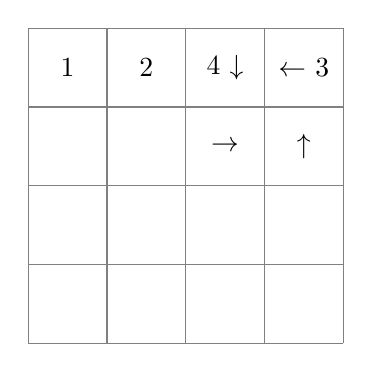
\begin{tikzpicture}
                \draw[step=0.5cm,color=gray,scale=2] (-1,-1) grid (1,1);
                \node at (-1.5,+1.5) {1};
                \node at (-0.50,+1.5) {2};
                \node at (+0.50,+1.5) {4 $\downarrow$};
                \node at (+1.5,+1.5) {$\leftarrow$ 3};
                \node at (-1.5,+0.5) {};
                \node at (-0.5,+0.5) {};
                \node at (+0.5,+0.5) {$\rightarrow$};
                \node at (+1.5,+0.5) {$\uparrow$};
                % ...
                \node at (+1.5,-1.5) {};
                
            \end{tikzpicture}
            \caption[Voorbeeld van Linear Conflict]{Toont een voorbeeldbord waar nummer 4 en 3 voor een Linear Conflict zorgen. Dit zorgt voor meer verplaatsingen dan andere zoals de pijlen aangeven.}
            \label{fig:Linear Conflicts}
        \end{figure}

        Wegens dit voor meer verplaatsingen zorgt, moeten we de kost hier ook op aanpassen. We doen dit door bij beide tegels hun manhattansom twee op te tellen. 
        Wanneer meerdere tegels zulk conflict hebben,
        kunnen we de tegel die het meeste verplaatsingen zou moeten doen eerst wegnemen. Zo minimaliseren we de andere conflicten en verplaatsingen. Dit alles vermindert het geheugengebruik en de uitvoeringstijd
        met een kleine factor die zichtbaar zal zijn, maar niet extreem groot zal zijn. Het nakijken van een Linear Conflict heeft een runningtime van $\sim n^3$ wegens we dit aantal moves moeten nakijken.
        \\
        \\Dit kunnen we opzichzelf nog eens verbeteren door enkel lijn conflicten na te kijken bij de betrokken kolom of rij loodrecht op de richting van de zet. Dit zorgt voor een runningtime van de linear conflicts van $\sim n^2$ in plaats van $\sim n^3$. 
    \pagebreak

    \subsection{Grotere puzzels}
    Zoals in \'e\'en van de eerste lessen gezien, een beter algoritme is vaak de beste keuze. Wegens we nu al enkele geoptimaliseerde structuren gebruiken, is de vraag of dit nog steeds geld.
    Wegens geheugen nu al snel een probleem is, kunnen we investeren in een computer met meer geheugen. Hier gaan we al snel tegen een muur botsten met een probleem met de tijd wegens deze niet versneld doordat we meer geheugen toevoegen.
    
    Wat we nu wel kunnen doen is gebruik maken van parallel programming. Voor alle mogelijke zetten, kunnen we een aparte thread toewijzen die dit efficient in parallel kan doen lopen.

    Deze optimalisatie zal uiteindelijke ook uren en langer draaien voor grotere en/of ingewikkeldere puzzels. Als we nu ook nog eens meer tijd zouden geven, is dit niet per se een probleem, maar dit loopt al snel naar de jaren, wat dan weer niet mogelijk is 
    wegens er nooit genoeg werkgeheugen kan bestaan.
    \\
    \\Hieruit valt af te leiden dat meer geheugen met een kleine optimalisatie al een mooi resultaat kan geven, maar dat het voor korte duur is. Dit komt door het feit dat
    er altijd minstens een keer over alle elementen in elk bord gelopen moet worden, en het aantal elementen per bord een grootteorde van $N^2$ hebben. Voor grote $N$ krijgen we een $NP$-probleem, wat op dit moment nog niet praktisch op te lossen is.

    \bibliographystyle{plain}
    \bibliography{bibliografie}

\end{document}
